\documentclass{article}

%change the margin of the paper
%\usepackage[legalpaper, margin=0.1in]{geometry}
\usepackage{amsmath}
% hyperlink Here
\usepackage{hyperref}
\hypersetup{
    colorlinks=true,
    linkcolor=blue,
    filecolor=magenta,
    urlcolor=cyan,
}

% this is the package for block comment \begin{comment} and \end{comment}
\usepackage{verbatim}
\usepackage{imakeidx}
% For multiple rows in tabular environment.
\usepackage{multirow}
% use this package to strikeout the word /st{}
%the color package is for the \textcolor{red} to highlight the text
\usepackage{color,soul}
% to define newcolumntype and \arraybackslash
\usepackage{array}
% hyperref is to call /url. hyphen packege to avoid that the url is too long
\PassOptionsToPackage{hyphens}{url}\usepackage{hyperref}
%Todo list, \newlist \setlist...
\usepackage{enumitem,amssymb}
\newlist{todolist}{itemize}{2}
\setlist[todolist]{label=$\square$}

% for image inserting
\usepackage{graphicx}
\graphicspath{./Desktop/Homework/123/5/}
\usepackage{subfig}

% \iff \leqlsant
\usepackage{amssymb}



% Code block begin(lstlisting) and end(lstlisting)
\usepackage{listings}
\usepackage{color}

\definecolor{dkgreen}{rgb}{0,0.6,0}
\definecolor{gray}{rgb}{0.5,0.5,0.5}
\definecolor{mauve}{rgb}{0.58,0,0.82}


%NOTE: Change the "language" parameter here
\lstset{frame=tb,
  language=Matlab,
  aboveskip=3mm,
  belowskip=3mm,
  showstringspaces=false,
  columns=flexible,
  basicstyle={\small\ttfamily},
  numbers=none,
  numberstyle=\tiny\color{gray},
  keywordstyle=\color{blue},
  commentstyle=\color{dkgreen},
  stringstyle=\color{mauve},
  breaklines=true,
  breakatwhitespace=true,
  tabsize=3
}

% Macros
%%%%%%%%%%%% Text Color %%%%%%%%%%%%%%%
\definecolor{mypink1}{RGB}{219, 48, 233}
\definecolor{myred1}{RGB}{231, 76, 60}
\definecolor{myred2}{RGB}{203, 67, 53}
\definecolor{myblue1}{RGB}{52, 152, 219}
\definecolor{mygray}{gray}{0.6}

%% Table Style
\newcolumntype{C}{>{\center\arraybackslash}m{.70\columnwidth}}
\newcolumntype{Y}{>{\center\arraybackslash}m{2cm}}




%NOTE title Here
\title{Math 123 Homework 5}
\author{Hanyuan Zhu}







\begin{document}
\maketitle

\subsection*{Question1}

\paragraph{(a)}

As $\epsilon \rightarrow \infty$ and $MinPts \leq n$ for dataset $ \{x_i\}^n_{i=1}$, the entire dataset become one cluster.

As $\epsilon \rightarrow +0$, and $MinPts \leq 1$, each point will become a single-point cluster; while the $MinPts \geq 2$, All points will become noisy points.

\paragraph{(b)}

As $MinPts \rightarrow \infty$, all points will be noises. No cluster will form.

As $MinPts \rightarrow +0$, all points are core points to form clusters, and no noise.



\subsection*{Question2}

\paragraph{(a)} Below is my function for DBSCAN algorithm. You can call it by DBSCAN(dataBase, eps, minPts), where dataBase is $n \times 2$ array, eps is the threshold of radius of corepoints neighorhood, and minPts is the minimum points in neighorhood qualified for corepoint.

It returns a $3 \times n$ matrix. The first two elements of each column representing a point, and the third element is the label of cluster of the point. The label of all noise point is $-1$ here.

\begin{lstlisting}
function [DB]=DBSCAN(dataBase, eps, minPts)

C = 0; % Cluster Counter

%% Prepare the Dataset
labelDB = zeros(length(dataBase),1);% Create a label set for DB
DB = [dataBase labelDB]';% transpose the DB, to make each vertical component of dataset as a point. for the "for loop" . Union the label and dataset
% NOTICE : Each column of DB is a point now

%% Preprocess the neigbhorhood set
DBdistance = pdist2(dataBase,dataBase);
NC = {};
toSearch = [];

%% to generate neighborhood matrix [[size of neighborhood, corepoint=1],[list
%of neigbhorhood index]]
for idx = 1:length(DBdistance)
    aa = find(DBdistance(:,idx)<eps & DBdistance(:,idx)>0);
    if length(aa) >= minPts
        NC{end+1} = {[length(aa),1],aa};
        toSearch(end+1) = idx;
    else
        NC{end+1} = {[length(aa),0],aa};
        DB(3,idx) = -1;
    end
end


%% Here only search all core points
while ~isempty(toSearch)
    idx = toSearch(1);
    toSearch(1) = [];

    if DB(3,idx)
        continue
    end

    C=C+1; % if P satisfies all conditions above, label lable it as a new cluster

    DB(3,idx)=C;
    seedSet= NC{idx}{2};

    while ~isempty(seedSet)
        idx = seedSet(1); % the index of such element in DB
        seedSet(1) = [];
        if DB(3,idx) == -1 %check if it is noise first. to update the label of noise point to border point
            DB(3,idx) = C;
        end

        if DB(3,idx) %skip all labelled point in neigbhorhood
            continue
        end

        seedSet = union(seedSet,NC{idx}{2});% adding the neighorhood of the idx core point to the seedset
        DB(3,idx) = C; % update the cluster label of idx point
    end

end
    scatter(DB(1,:),DB(2,:),25,DB(3,:),'filled')
end

\end{lstlisting}

\paragraph{(b)}
I run the following code block to to try different values of eps and minPts
\begin{lstlisting}
load("DBSCAN_Data.mat");

%fixing the minPts for various eps.
DBSCAN(X,0.02,5);
DBSCAN(X,0.05,5);
DBSCAN(X,0.1,5);
DBSCAN(X,0.2,5);

%fixing the eps for various minPts.
DBSCAN(X,0.05,2);
DBSCAN(X,0.05,5);
DBSCAN(X,0.05,10);
DBSCAN(X,0.05,50);
DBSCAN(X,0.05,51);
\end{lstlisting}


\begin{figure}[h]
  \centering
  \subfloat[ eps=0.02 ]{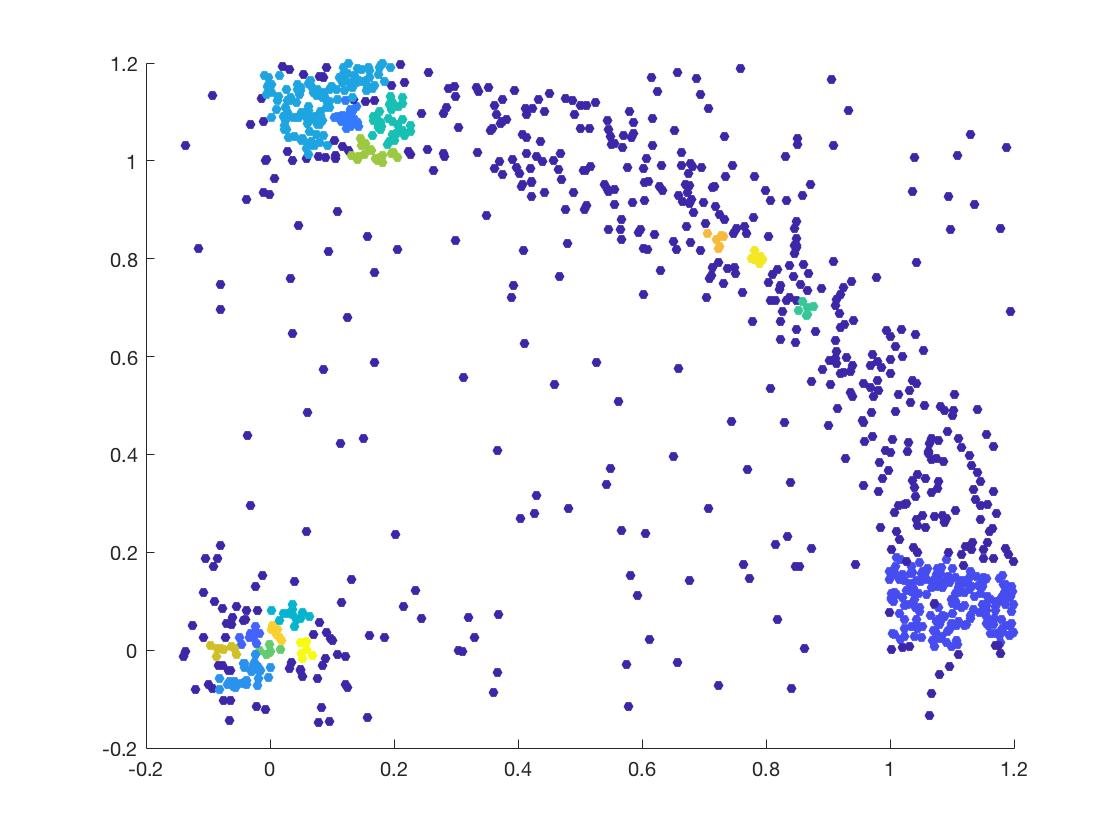
\includegraphics[width=3cm, height=3cm]{002_5}}
  \qquad
  \subfloat[ eps=0.05 ]{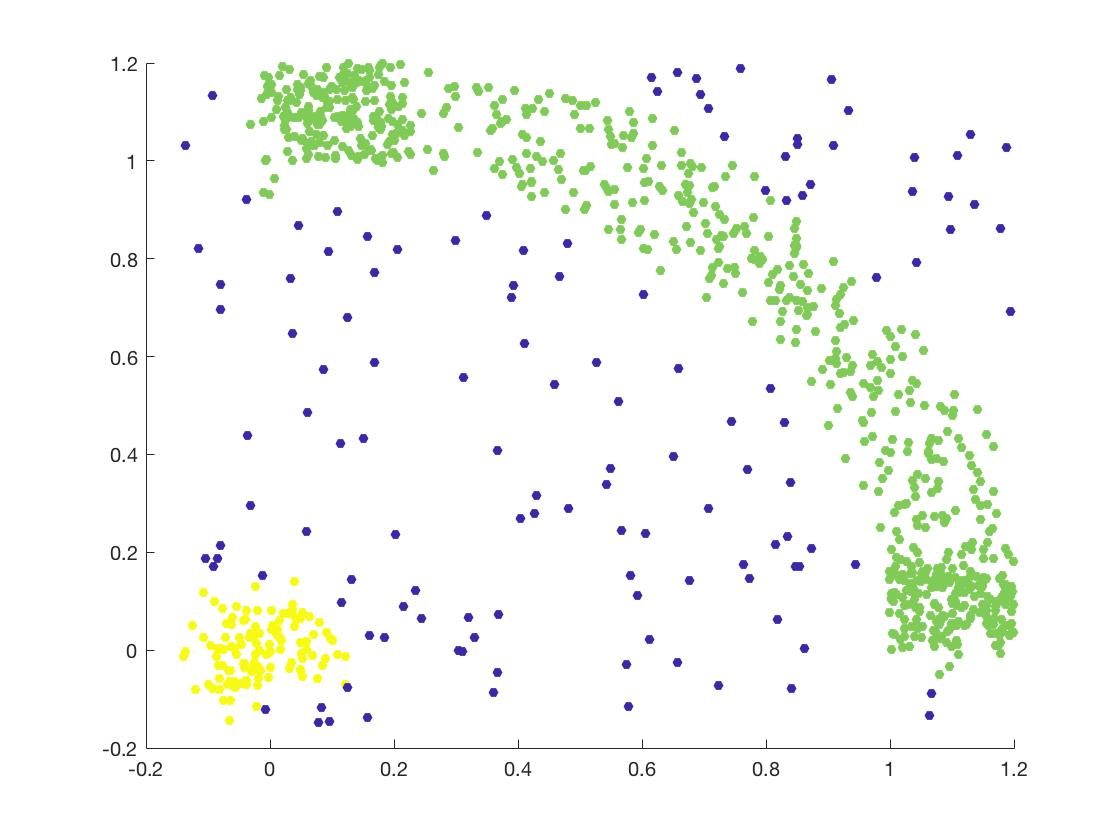
\includegraphics[width=3cm, height=3cm]{005_5}}
\end{figure}

\begin{figure}[h]
  \centering
  \subfloat[eps=0.1]{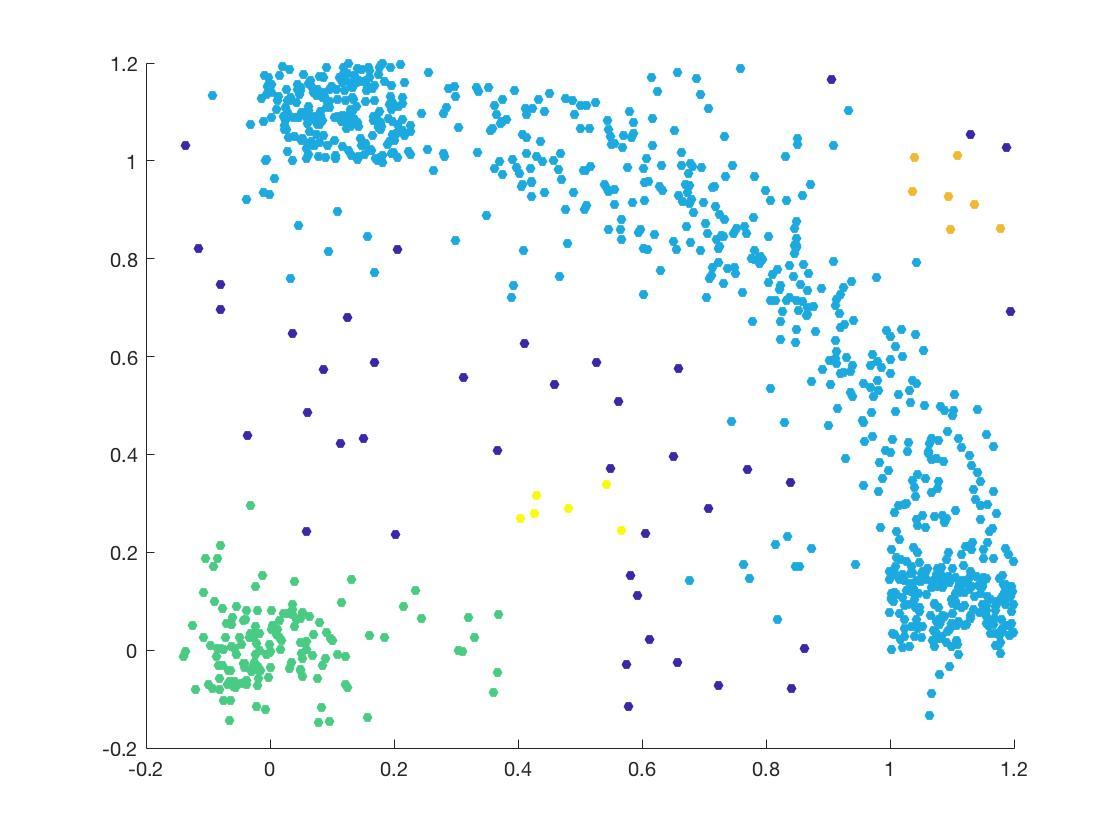
\includegraphics[width=3cm, height=3cm]{01_5}}
  \qquad
  \subfloat[eps=0.2 ]{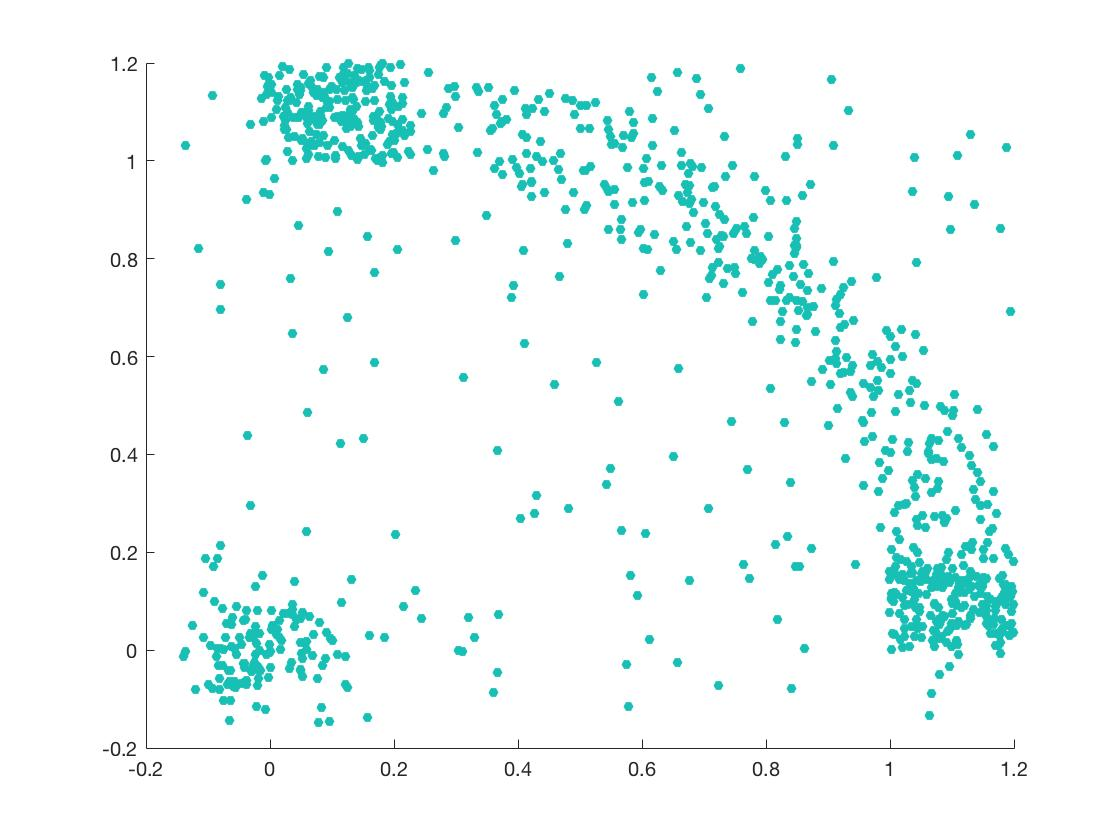
\includegraphics[width=3cm, height=3cm]{02_5}}
  \caption{Fixing the mintPts = 5}
\end{figure}


\begin{figure}[h]
  \centering
  \subfloat[ minPts = 2 ]{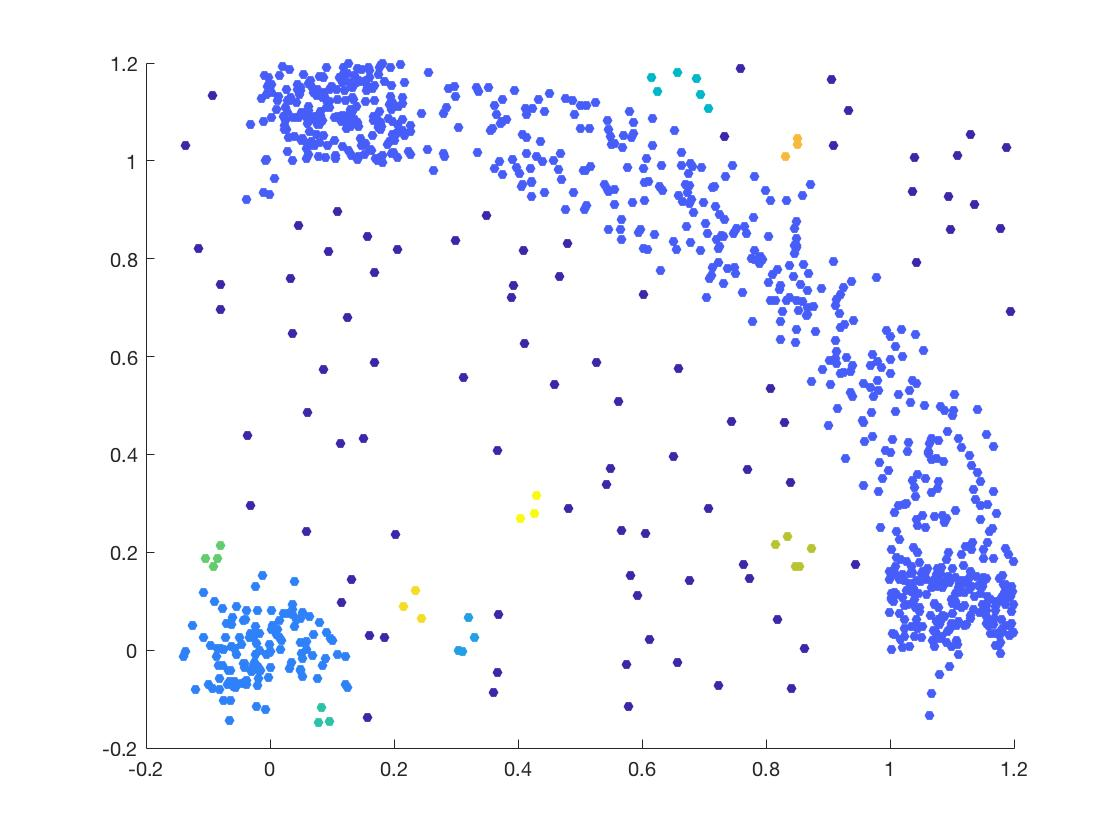
\includegraphics[width=3cm, height=3cm]{005_2}}
  \qquad
  \subfloat[ minPts = 5 ]{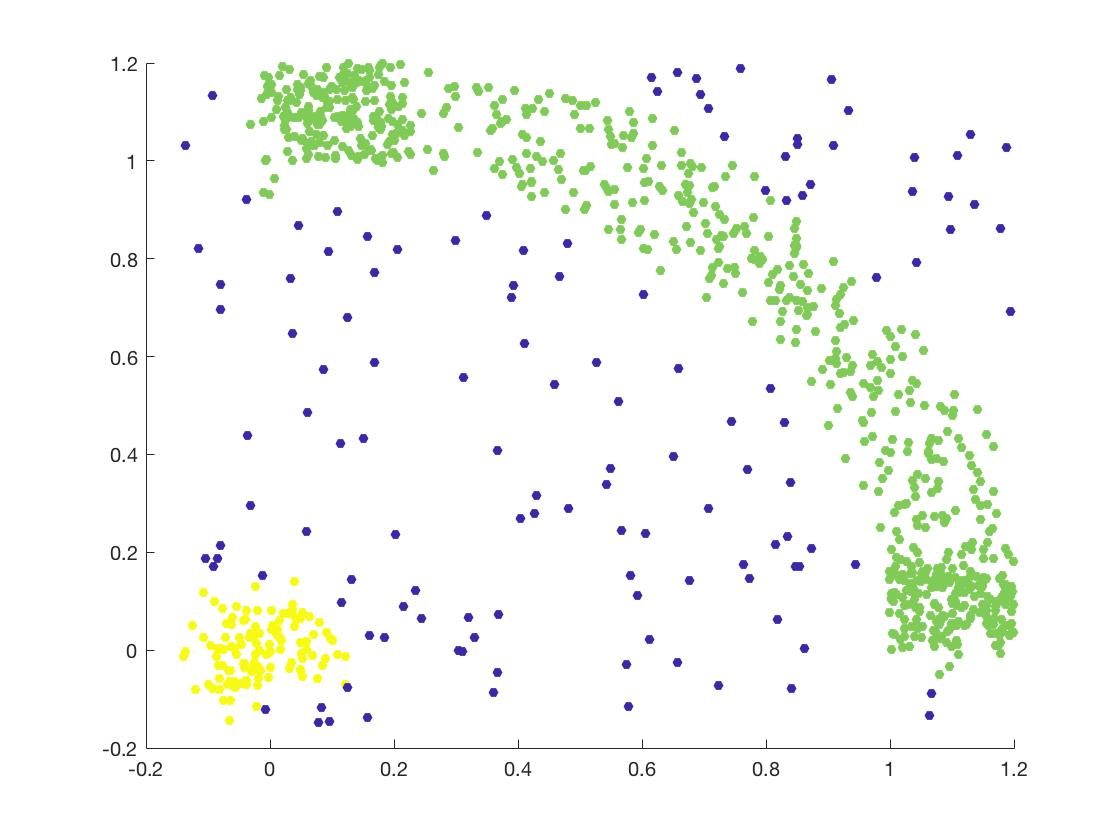
\includegraphics[width=3cm, height=3cm]{005_5}}
  \qquad
  \subfloat[ minPts = 10 ]{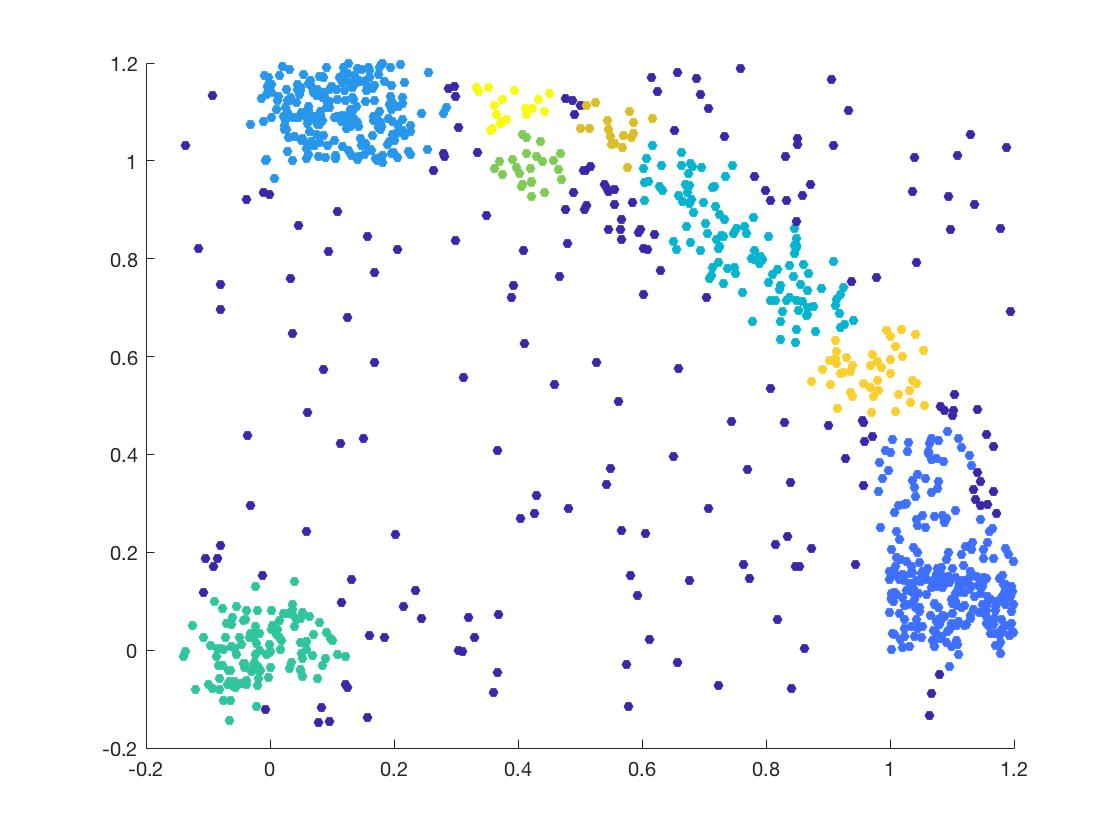
\includegraphics[width=3cm, height=3cm]{005_10}}
\end{figure}

\begin{figure}[h]
  \centering
  \subfloat[ minPts = 50 ]{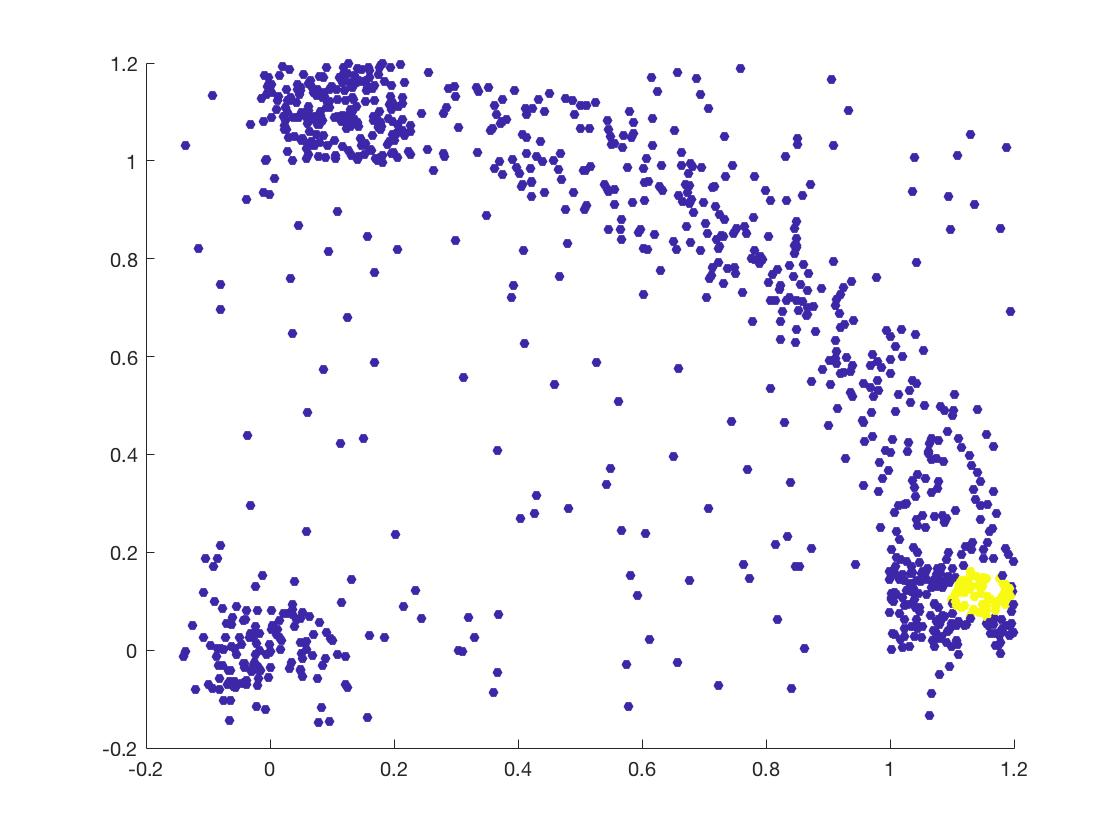
\includegraphics[width=3cm, height=3cm]{005_50}}
  \qquad
  \subfloat[ minPts = 51 ]{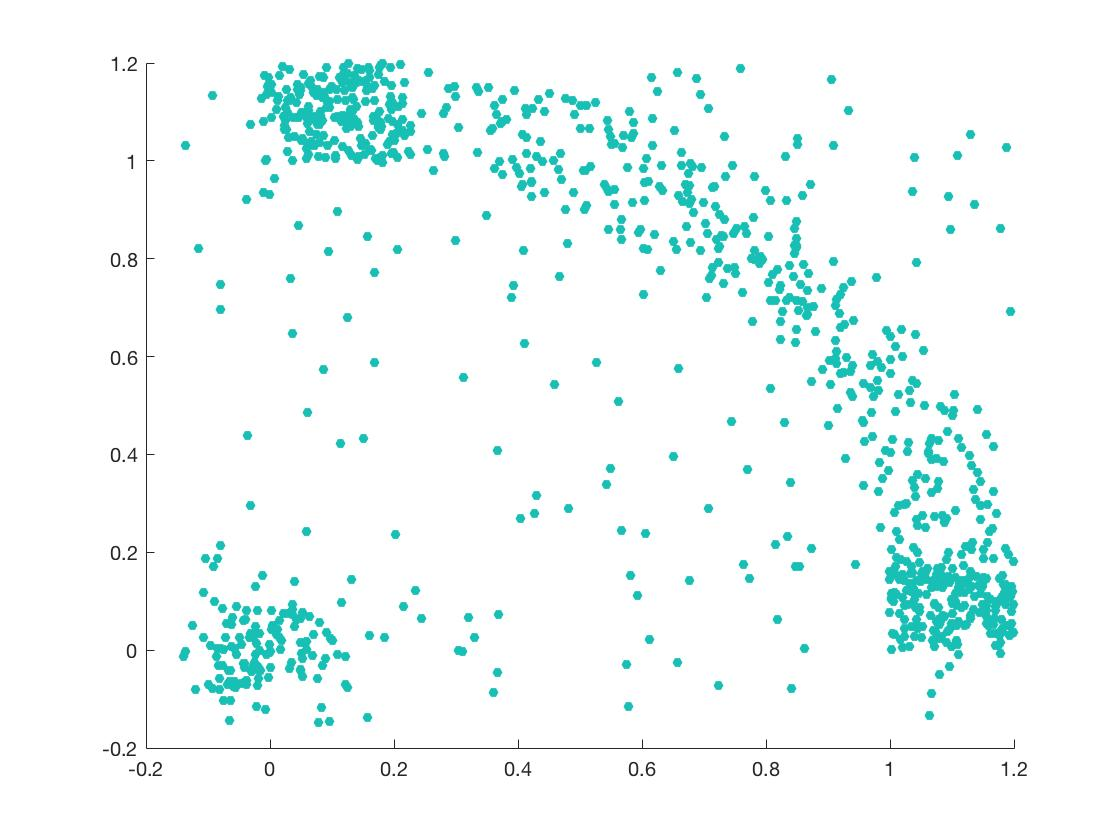
\includegraphics[width=3cm, height=3cm]{005_51}}
  \caption{Fixing the eps = 0.05}
\end{figure}

\newpage

Clearly, the relatively best partition result is at eps = 0.05 and minPts = 5.

The DBSCAN fails at eps larger than 1.5(for fixing minPts=5), where more and more noise points will be included.

The DBSCAN completely fails at minPts larger than 50(for fixing eps=0.05), where all points are counted as noise.



\subsection*{Question3}

\paragraph{(a)}
To show L is positive semidefinite, that is, to show $yLy^T \geq 0$ for any $y \in \mathbb{R}^{1\times n}$, $y \neq 0$

Because $ L = D - W $,

\begin{equation}
  \begin{split}
  yLy^T & = \sum^n_{i=1} \sum^n_{j=1} L_{ij} y_i y_j\\
  & = \sum^n_{i=1} \sum^n_{j=1} (D_{ij}-W_{ij}) y_i y_j\\
  & = \sum^n_{i=1} \sum^n_{j=1} D_{ij} y_i y_j - \sum^n_{i=1} \sum^n_{j=1} W_{ij} y_i y_j\label{eq:1}
\end{split}
\end{equation}

Since $D_{ij} = 0, if i \neq j$ and $ D_{ii} = \sum^n_{j=1} W_{ij}$, also by relabeling the index, we have $ \sum^{n}_{i=1} D_{ii} y^{2}_{i} = \sum^{n}_{j=1} D_{jj} y^{2}_{j} = \sum^{n}_{i=1} \sum^n_{j=1} W_{ij} y^{2}_{j}$
 then

\begin{equation}
  \begin{split}
  (1) & = \sum^n_{i=1} D_{ii} y^2_{i} - \sum^n_{i=1} \sum^n_{j=1} W_{ij}  y_i y_j\\
  & = \frac{1}{2} ( 2 \sum^n_{i=1} D_{ii} y^2_{i} - 2 \sum^n_{i=1} \sum^n_{j=1} W_{ij} ) \\
  & = \frac{1}{2} ( \sum^n_{i=1} D_{ii} y^2_{i} + \sum^n_{j=1} D_{jj} y^2_{j} - 2 \sum^n_{i=1} \sum^n_{j=1} W_{ij} ) \\
  & = \frac{1}{2} (\sum^n_{i=1} \sum^n_{j=1} W_{ij}  y^2_{i} + \sum^n_{i=1} \sum^n_{j=1} W_{ij}  y^2_{j} - 2 \sum^n_{i=1} \sum^n_{j=1} W_{ij}  y_i y_j)\\
  & = \frac{1}{2} \sum^n_{i=1} \sum^n_{j=1} W_{ij} ( y^2_{i} +  y^2_{j} - y_i y_j )\\
  & = \frac{1}{2} \sum^n_{i=1} \sum^n_{j=1} W_{ij} ( y_{i} -  y_{j})^2 \label{eq:2}
\end{split}
\end{equation}

Because  $W_{ij} \in [0,1]$ and $( y_{i} -  y_{j})^2 \geq 0 $, then
\begin{equation}
  yLy^T = \frac{1}{2} \sum^n_{i=1} \sum^n_{j=1} W_{ij} ( y_{i} -  y_{j})^2 \geq 0
\end{equation}

Thus $L$ is positive semidefinite matrix.

\paragraph{(b)}
Because $L$ has a eigenvalue 0, that is, $ v^{T}Lv = 0$, where $v$ is the eigenvector of eigenvalue 0, and $v \neq 0$. Therefore $L$ is not positive definite.


\subsection*{Question4}



\begin{figure}[h]
  \centering
  \subfloat{
\includegraphics[height=3cm]{sigma02}}
  \qquad
  \subfloat{
\includegraphics[height=3cm]{sigma05}}
  \qquad
  \subfloat{
\includegraphics[height=3cm]{sigma1}}
  \qquad
  \subfloat{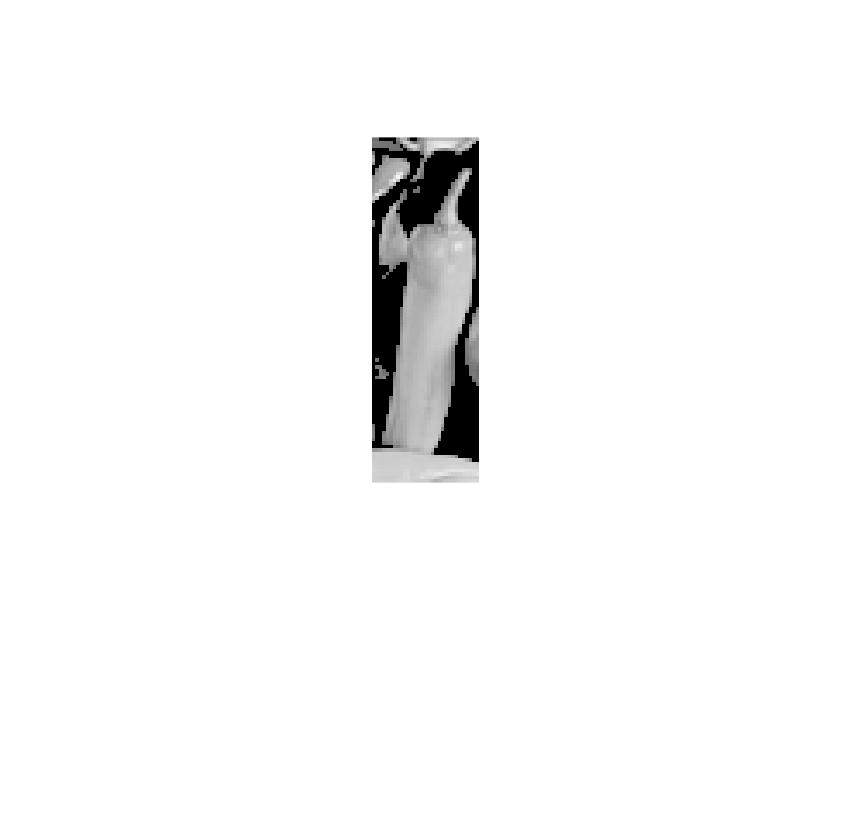
\includegraphics[height=3cm]{sigma5}}
  \caption{from top to bottom right, $\sigma$ are 0.2, 0.5, 1 and 5}
\end{figure}

Because the weight function is determined by the difference of the color (or brightness) of two pixel points, thus when the $\sigma$ becomes sufficiently large, the color (or brightness) between two pixels are become smaller or even neglectible.

Therefore, as the $\sigma$ go larger, the wider color range will be shown on the results.
\newpage
\subsubsection*{The code for graph Lapacian}
\begin{lstlisting}
load('Ncut_Data.mat')
reshaped = reshape(pepper,[], 1);

% Wdist is the matrix of the 2 norm of x_i and x_j
Wdist = pdist2(reshaped,reshaped);

%set sigma here
sigma = 0.2;
sigM = ones(size(Wdist))*sigma;

% here is the weight matrix
W = arrayfun(@expoweight, Wdist, sigM);

%sum each column of W, to get the D_i. and diagnolize the vector.
D =diag(sum(W,2));

%graph Lapacian = D - W
L = D - W;

%eigenvlaue decomposition
[V E] = eig(L);

% Since the eigenvalue is sorted. the second smallest is E(2,2), and the
% vector is V(:,2)

%processing the data

imagebyV = arrayfun(@bipartitioN,reshaped,V(:,2));

newpepper = reshape(imagebyV,100,31);

imshow(newpepper)



\end{lstlisting}


\end{document}
